\chapter{Phase 4 --- Further UI/UX Iteration}
\section{Requirements Analysis}
This phase was time limited, as the project was nearing its end. For this reason, this phase was mostly focused on fixing the high priority issues identified in the previous phase. This included adding a light mode, adding syntax highlighting, as well as fixing language and typechecker bugs. 

At the end of this phase, I wanted to hold another focus group where Amos would give a lecture on functional programming, but this time to complete beginners. After a planning conversation with Amos at the beginning of Phase 4, we identified that it would be useful to add an `untyped mode' so the beginners could be taught the basics of \lcalc\ before trying to explain types, as they can be initially confusing. 

\section{Design and Implementation}
\subsection{Syntax Highlighting}
In order to implement syntax highlighting, I found the source code for the Haskell syntax highlighting supported by the library I was using for my editor (\href{https://codemirror.net/5/}{CodeMirror 5}). I edited this with SFL's syntax and keywords. Syntax highlighting was also applied to the prelude to make it easier to read. 

\subsection{Light Mode, and the Settings Menu}
The `light mode' colour scheme was designed by returning to the room where the Intermediate Focus Group was held on a day with similar amounts of sunshine, and testing different colours for visibility. The light mode scheme also had different syntax highlighting from dark mode. See figure~\ref{fig:screenshot_final_light_1} for a screenshot. 

\begin{figure}[h]
    \centering
    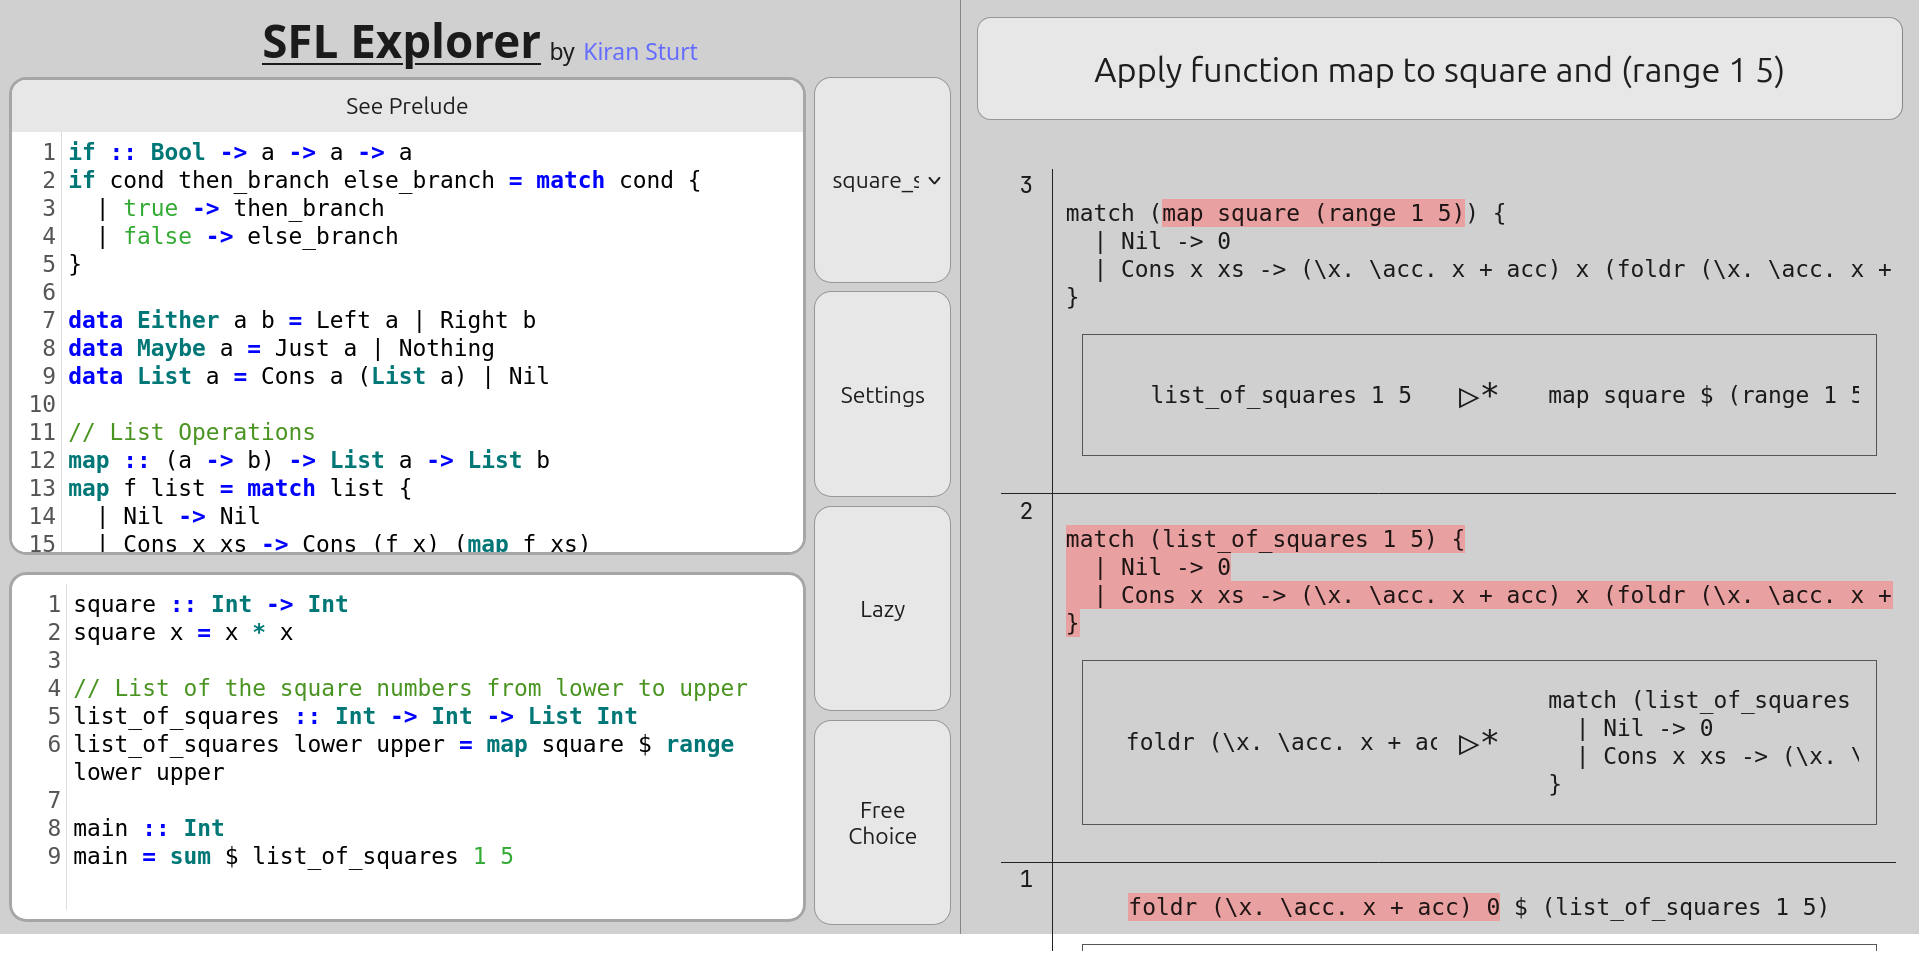
\includegraphics[width=\linewidth]{images/final_light_3.png} 
    \captionsetup{justification=centering}
    \caption{The final product during lazy evaluation of the `sum of squares' sample program in light mode}
    \label{fig:screenshot_final_light_1}
\end{figure}

To implement it, I added a floating settings menu with a button that would toggle from light mode to dark mode. This worked by adding or removing the class `light' from the top level HTML element, where all elements descending from this node would be in light mode if it was set. I also added a button for toggling `untyped mode', as well as toggling whether the prelude was included. These settings would be saved in the user's browser.

Using CSS media queries, I was also able to tell the user's preference for light or dark mode from their browser, and use this by default unless the user chose otherwise. 

% \subsection{Bugfixes}
% \subsubsection{Frontend}

\section{The Beginner Focus Group: Evaluation and Next Steps}
\label{eval:BFG}
\subsection{Selection and Format}
This focus group had the same format as the intermediate focus group \ref{eval:IFG}; Amos was employed once more to give a 45-minute lecture, followed by a 45-minute interview. The full transcript of the lecture and interview is available in the auxiliary materials \ref{appx:additional_mats}.

The goal of this focus group was to evaluate the use of SFL explorer in a lecture setting with complete beginners, with a wide variety of different experiences with and perspectives on programming. Crucially, I wanted none of them to have learnt about or used functional languages before. As such, I decided to recruit non computer scientists. In order to get a mix of more `practical' and more `theoretical' students, the four students I recruited had the following backgrounds:

\begin{itemize}
    \item A second year undergraduate Mechanical and Aerospace Engineer from the University of Cambridge, with experience in Python, C/C++.
    \item A third year undergraduate Mechanical Engineer from the University of Bristol, with experience in Python and C/C++.
    \item Two third year undergraduate Maths students from the University of Bristol, with experience in mostly Python and R.
\end{itemize}

\subsection{Bugs}
There was a bug where the type checker would not correctly follow type aliases, causing crashes in a program with type aliases. This was fixed afterwards. 

\subsection{Outcomes}

\subsubsection{The Language}
Participant's did not have many comments on the language, as they had never seen a functional language before, so they couldn't really compare. However, Participant 2 (a Maths student) in particular seemed excited about functional programming as a concept:
\begin{quotation}
\noindent `It's cool to see a language that's like, I don't know, I feel like if I was going to do some maths in my head, this is how I'd actually do it' [Participant 2, 01:05:22]. 
\end{quotation}
\noindent Participant 2 also asked several questions about the history of functional programming, showing their engagement. 
% Participant 1 was confused about the bar character used to separate cases in a match statement, as it was the same as the character used to separate tagged union variants. 

\subsubsection{The User Interface, and the System as a Whole}
Most of the feedback was positive, and users had no specific feedback on what they would like to see be changed in the system. 

\begin{itemize}
    \item Two participants said they preferred dark mode, but both agreed light mode is important to have.
    
    \item Free choice mode was very popular, with two participants specifically mentioning when asked for things they liked in the system. 

    \item Participant 3 really liked the interface, and found the session particularly interesting:
    
    `I really like the coding part and the sections on the right, in terms of seeing how it goes from one to another. I think that was really useful. In terms of learning it. Yeah. And the free choice variation. I also agree that it shows nicely what the functions are actually doing' [Participant 3, 01:03:11]

    \item Participant 2, a Maths student, was very positive about the UI and the tool:
    
    `I think you've done a really good job of making it quite beginner-friendly because it's all quite easy to read' [Participant 2, 01:06:05]

    \item `UX is very intuitive' [Participant 1, 01:12:07]
\end{itemize}

\section{The Final Client Meeting}
\label{c4:client}
After the beginner focus group, I met my client, Samantha Frohlich, in order to evaluate the project. We discussed how useful the finished product would be for teaching functional programming~(see~\ref{c4:client}). She concluded that it would be very useful, and she plans to integrate it into the first year functional programming course~\hyperref[COMS10016]{COMS10016} in following years. 

Following this meeting, my client shared the project with Jamie Willis, a teaching fellow at Imperial College London, who is involved in their first year unit which includes functional programming \cite{imperialFP}. When my client asked Jamie about whether he would use it, he responded:

\begin{quotation}
\noindent `I could see it being useful for sure, a lot of the time I end up writing out these step-by-step reductions by hand in my notes, but it would be nice for them to have access to a tool they could use to explore for themselves'
\end{quotation}

\paragraph{The Language}
Samantha was very positive about the language. More specifically, she liked the following things:

\begin{itemize}
    \item The language is minimal and clear, and it has the right set of features for the purpose it is designed for and no more.
    \item The type system is sufficient to express complex programs. Type aliases and data types are defined using Haskell syntax. 
    \item Pattern matching is very clear, and she agreed with all three focus groups that it is good for a teaching tool. 
    \item The type checker is robust; she was not able to break it. 
    \item Untyped mode is very useful to have, especially for demonstrating the untypable Y-combinator
    \item The provided examples were useful. 
    \item The prelude was good, and she could not think of anything else she would want to add to it. 
\end{itemize}

\noindent She had the following feedback about the language:

\begin{itemize}
    \item Even though \lcalc\ abstractions are typically expressed like \verb|\x. M| with a dot separating the variable and the term, she thought it should be an arrow in \ac{SFL} to match Haskell.
    \item She identified, like the advanced focus group did, that expressions often balloon very quickly into a series of nested matches. This is definitely a weakness of the project, and it is something to be improved on~\ref{conc:baboon}.
    \item She thought that \sflinline{Cons} should be an infix operator \sflinline{:}. However, after discussing the results of the advanced~\ref{ref:afg} and intermediate~\ref{eval:IFG} focus groups with her, and how the consensus in these groups was that explicitly writing \sflinline{Cons} was clearer, she changed her mind. 
\end{itemize}

\paragraph{UI/UX and the System as a Whole}
She was also very positive about the UI/UX and the system as a whole. She mentioned liking the following things:

\begin{itemize}
    \item The UI looks nice, very practical.
    \item The syntax highlighting was good
\end{itemize}

\noindent The only specific thing she mentioned wanting changed was she wanted to be able to use the keyboard to control progress, for instance using the `up' and `down' keys for forward and backwards.

% `Wait, is SFL your language? It was so good that i just assumed you had grabbed it from somewhere'

% The aims of this focus group were to use the system and attempt to recap functional programming concepts 

% Evaluation:
% - They liked explicit match: they liked it more than Haskell for learning about how pattern matching works
% - Really Really needed light mode
% - Horizontal overflow bug

% A/B testing different schemes with some of my fellow undergraduates, as 

% The changes to the UI were time-consuming but not worth mentioning here. 